\documentclass[10pt]{beamer}

\beamertemplatenavigationsymbolsempty
\renewcommand\mathfamilydefault{cmr}

\usepackage{pajmath}
\usepackage{booktabs}
\usepackage{colortbl}

\usepackage{tikz}
\usetikzlibrary{positioning,shapes.misc,calc,backgrounds,scopes} 
\usetikzlibrary{datavisualization}
\usetikzlibrary{datavisualization.formats.functions}
\tikzset{boxed/.style={
  thick,
  draw=black,
  top color=white,
  text height=1.5ex,
  text depth=.25ex
}}


\newcommand\lo{\ensuremath{\boldsymbol{-}}}
\newcommand\hi{\ensuremath{\boldsymbol{+}}}

\title{Response Surface Methodology:\\Optimizing Second-Order Models}
\author{BIOE 498/598 PJ}
\date{Spring 2021}

\begin{document}
\frame{\titlepage}

\begin{frame}{Second-order response surfaces: Maximum}
	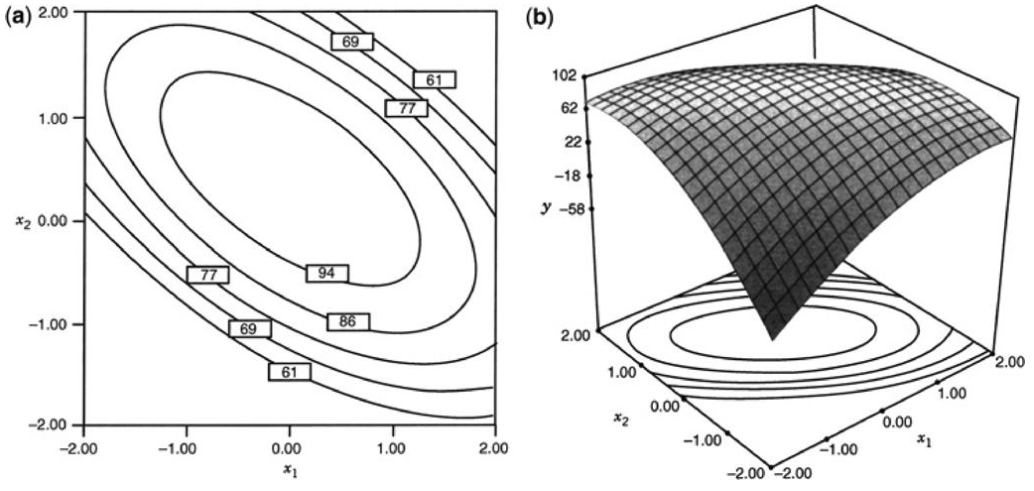
\includegraphics[width=\textwidth]{figures/rsm_maximum}
\end{frame}

\begin{frame}{Second-order response surfaces: Minimum}
	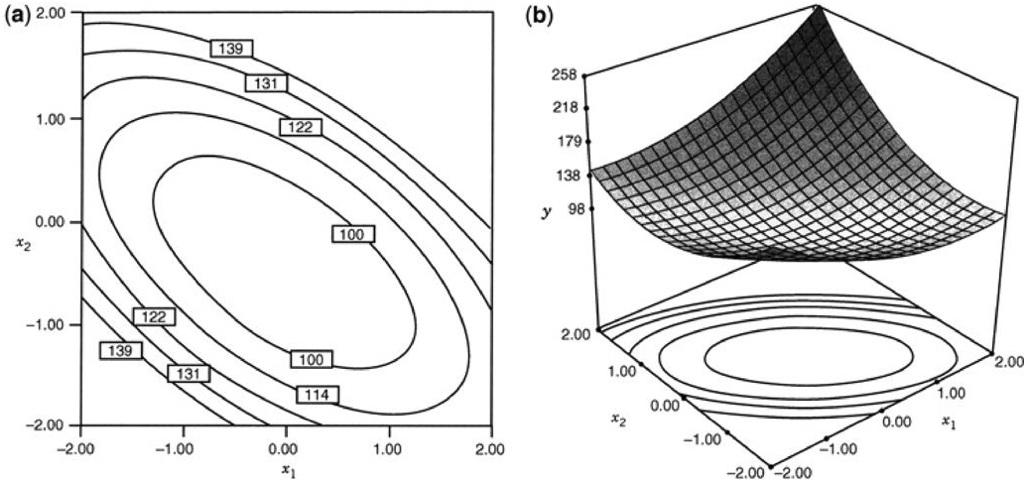
\includegraphics[width=\textwidth]{figures/rsm_minimum}
\end{frame}

\begin{frame}{Second-order response surfaces: Saddle Point}
	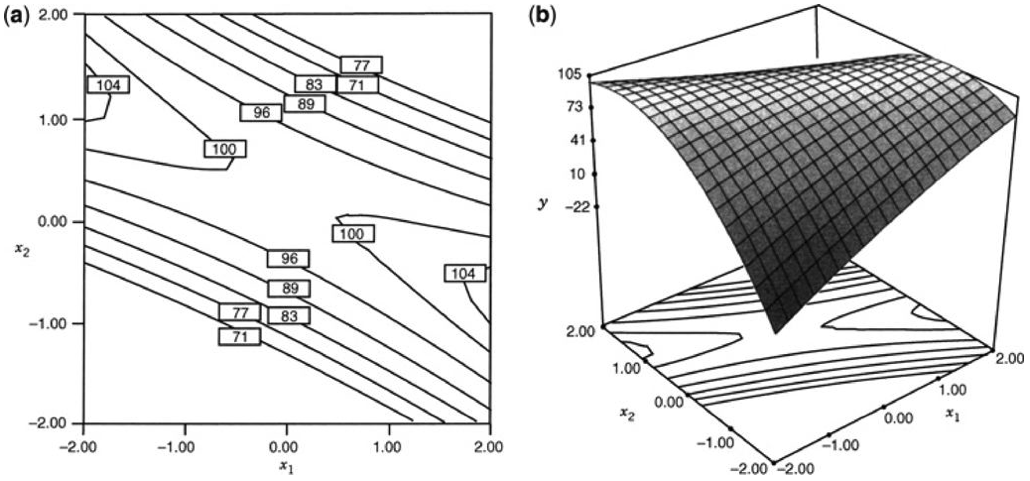
\includegraphics[width=\textwidth]{figures/rsm_saddle}
\end{frame}

\begin{frame}{Finding the response stationary point}
The general second-order linear model is
\[ y = \beta_0 + \sum_{i=1}^k\beta_ix_i + \sum_{i=1}^k\beta_{ii}x_i^2 + \sum_{j=1}^k\sum_{i=1}^{j-1}\beta_{ij}x_ix_j. \]

\pause
We can rewrite this using matrix notation:
\[ y = b_0 + \transpose{\Vx}{\Vb} + \transpose{\Vx}\VB\Vx. \]

\[ b_0 = \beta_0, \quad \Vb = \begin{pmatrix}\beta_1\\ \vdots \\ \beta_k \end{pmatrix}, \quad \VB = \begin{pmatrix} \beta_{11} & \beta_{12}/2 & \cdots & \beta_{1k}/2 \\ & \beta_{22} & \cdots & \beta_{2k}/2 \\ & & \ddots & \vdots \\ \mathrm{sym} & & & \beta{kk} \end{pmatrix} \]

\pause
\[ y = 3 - 0.3x_1 + x_2 + 1.2x_1^2 - 0.4x_1x_2 \]
\[ b_0 = 3,\quad \Vb = \vectwo{-0.3}{1},\quad \VB = \begin{pmatrix} 1.2 & -0.2 \\ -0.2 & 0 \end{pmatrix} \]
\end{frame}

\begin{frame}{Where is the stationary point?}

The argmin, argmax, or inflection point of a saddle is called the \textbf{stationary point} ($\Vx_s$).

\pause
\begin{align*}
	\frac{\partial y}{\partial \Vx} &= \frac{\partial}{\partial \Vx}\left(b_0 + \transpose{\Vx}\Vb + \transpose{\Vx}\VB\Vx \right) \\
		&= 	\Vb + 2\VB\Vx 
\end{align*}

\pause
Solving for where the derivative equals zero:
\[ \Vb + 2\VB\Vx_s = \Vzero \Rightarrow \Vx_s = -\frac{1}{2}\VB^{-1}\Vb \]
	
\end{frame}

\begin{frame}{What is the response at the stationary point?}

\begin{align*}
	y_s &= b_0 + \transpose{\Vx_s}\Vb + \transpose{\Vx_s}\VB\Vx_s \\
		&= b_0 + \transpose{\Vx_s}\Vb + \left(-\frac{1}{2}\transpose{\Vb}\VB^{-1}\right)\VB\Vx_s \\
		&= b_0 + \frac{1}{2}\transpose{\Vx_s}\Vb
\end{align*}

\pause
The response at the stationary point only depends on the intercept and the main effects.

\pause
\bigskip
\begin{columns}
\begin{column}{0.5\textwidth}
	Imagine a downward facing parabola \[y = 3 - (x-3)^2.\]
	
	The argmax is $x_s=3$ with response 
	\begin{align*} 
		y_s &= 3 - (3-3)^2 \\
		 &= 3 - 0^2.
	\end{align*}
\end{column}	

\begin{column}{0.5\textwidth}
	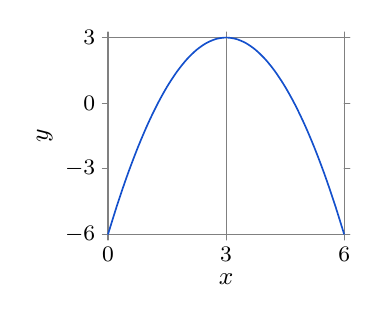
\begin{tikzpicture}
		\def\xlen{3cm}
		\def\ylen{2.5cm}
		\datavisualization [
			scientific axes, 
			x axis={length=\xlen, ticks={step=3}, label={$x$}},
			y axis={length=\ylen, ticks={step=3}, label={$y$}},
			visualize as smooth line,
			style sheet=vary hue]
		data [format=function] {
			var x : interval [0:6];
			func y = 3 - (\value x-3)*(\value x-3);
		};
		\draw [help lines] (1.5,0) -- (1.5,2.5);
	\end{tikzpicture}
\end{column}	
\end{columns}	
\end{frame}

\begin{frame}{Chemical Process Example (Myers 2016)}

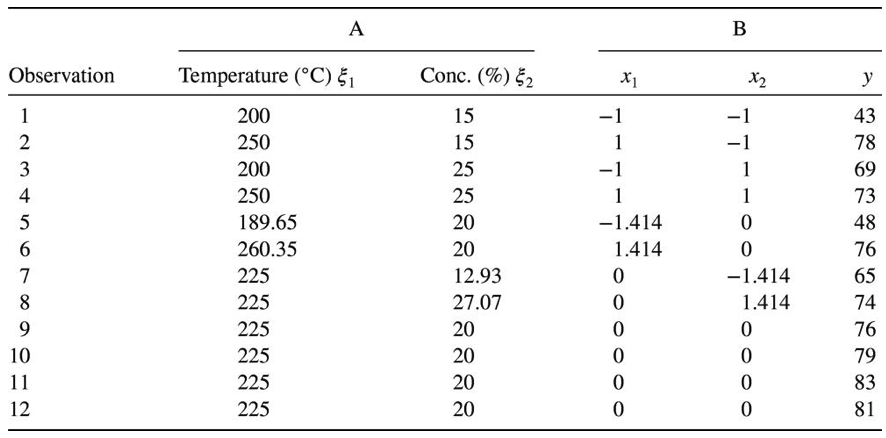
\includegraphics[width=\textwidth]{figures/rsm_chemical.png}
	
\pause
\[ y = 79.75 + 10.18x_1 + 4.22x_2 - 8.50x_1^2 - 5.25x_2^2 - 7.75x_1x_2 \]
\end{frame}

\begin{frame}{Chemical Process Example (Myers 2016)}

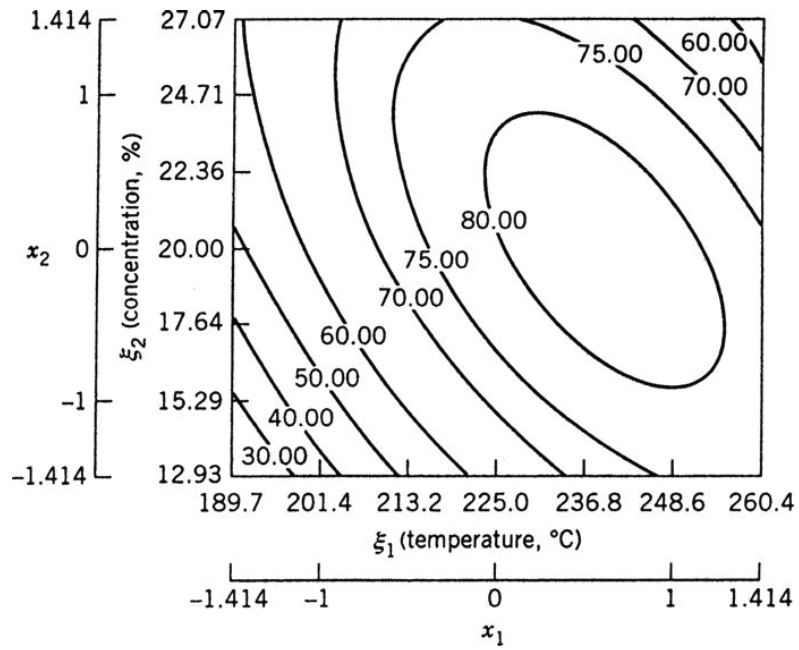
\includegraphics[width=0.8\textwidth]{figures/rsm_chemical_contour.png}
	
\[ y = 79.75 + 10.18x_1 + 4.22x_2 - 8.50x_1^2 - 5.25x_2^2 - 7.75x_1x_2 \]
\end{frame}

\begin{frame}{Where is the stationary point?}
\[ y = 79.75 + 10.18x_1 + 4.22x_2 - 8.50x_1^2 - 5.25x_2^2 - 7.75x_1x_2 \]
\pause
\[ b_0=79.75,\quad \Vb=\vectwo{10.12}{4.22},\quad \VB = \begin{pmatrix} -8.50 & -3.875\\-3.875 & -5.25 \end{pmatrix} \]

\pause
\begin{align*}
		\Vx_s &= -\frac{1}{2}\VB^{-1}\Vb \\
		&= -\frac{1}{2}\begin{pmatrix}-0.1773&\phan0.1309\\\phan0.1309&-0.2871\end{pmatrix}\vectwo{10.12}{4.22} \\
		&= \vectwo{0.6264}{-0.0604}
\end{align*}

\pause
\medskip
Temperature $= 225 + 25x_{1,s} = 225+25(0.6264) = 240^\circ$C

\medskip
Concentration $=20 + 5x_{2,s} = 20+5(-0.0604) = 19.7$\%

\end{frame}

\begin{frame}{Visual confirmation of stationary point}

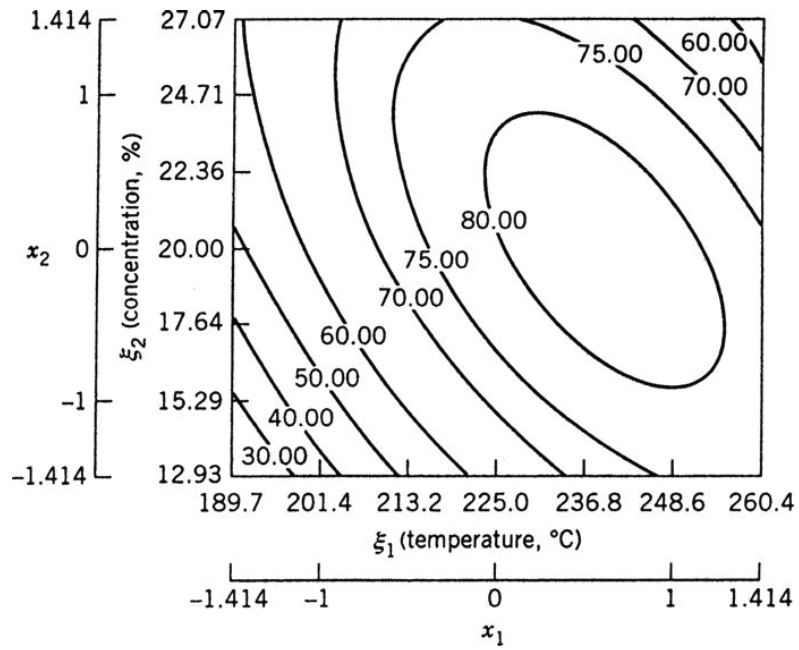
\includegraphics[width=0.8\textwidth]{figures/rsm_chemical_contour.png}

Temperature $= 240^\circ$C

\medskip
Concentration $= 19.7$\%
	
\end{frame}

\begin{frame}{When does $\Vx_s$ produce a maximum?}

\begin{itemize}
	\item The stationary point can be an argmax, argmin, or location of a saddle point.
	\item<2-> The type of extremum is determined by the eigenvalues ($\lambda_i$) of the matrix $\VB$.
		\begin{itemize}
			\item All $\lambda_i < 0 \rightarrow$ maximum
			\item All $\lambda_i > 0 \rightarrow$ minimum
			\item Indeterminate signs $\rightarrow$ saddle point
		\end{itemize}
	\item<3-> In the previous example, $\lambda_1=-11.0769$ and $\lambda_2=-2.6731$, so $\Vx_s$ is an argmax.
\end{itemize}
	
\end{frame}

\begin{frame}{*Canonical analysis}
We can simplify analysis by shifting our coordinates to the stationary point and rotating the axes to align with the eigenvectors.

\pause
\medskip
Let $\VV$ be a matrix with columns equal to the eigenvectors of $\VB$, and let
\begin{align*}
	\Vz &= \Vx - \Vx_s \\
	\V{w} &= \transpose{\VV}\Vz	
\end{align*}

\pause
The response anywhere can be defined in terms of the \textbf{canonical vector} $\V{w}$ an a diagonal matrix of eigenvalues $\V{\Lambda}$,
\[ y = y_s + \transpose{\V{w}}\V{\Lambda}\V{w} \]
\pause
or, more simply,
\[ y = y_s + \sum_{i=1}^k \lambda_i w_i^2 \]
\end{frame}

\begin{frame}{*Canonical analysis}
\begin{columns}
\begin{column}{0.3\textwidth}
	\[ \V{w} = \transpose{\VV}(\Vx - \Vx_s) \]
	\[ y = y_s + \sum_{i=1}^k \lambda_i w_i^2 \]
\end{column}
\begin{column}{0.7\textwidth}
	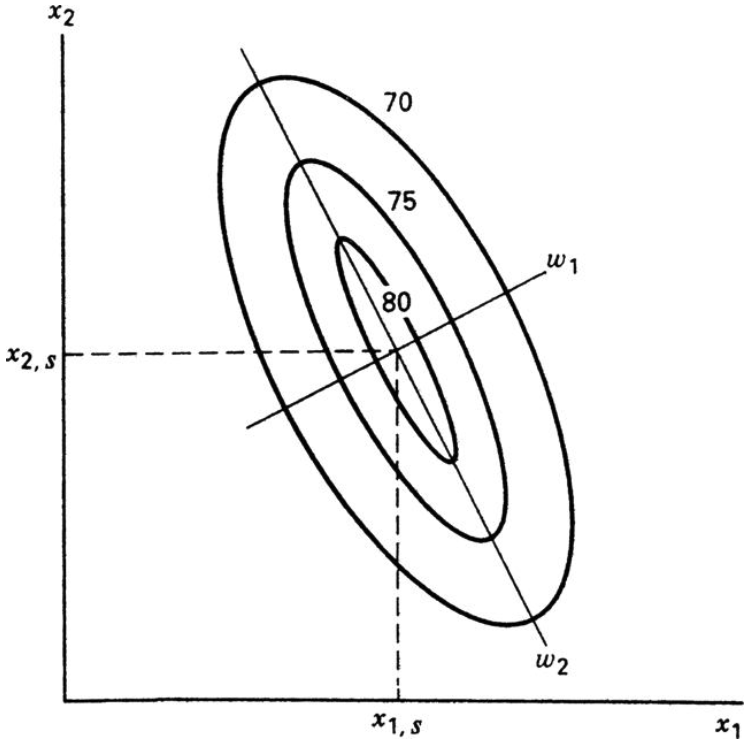
\includegraphics[width=\textwidth]{figures/rsm_canonical_analysis}
\end{column}
\end{columns}	
\end{frame}


\end{document}
